\documentclass[11pt, pdftex]{article}
\usepackage[margin=1in]{geometry}
\usepackage{graphicx}
\usepackage{amsmath}
\usepackage{listings}
\usepackage{semantic}
\usepackage[hyphens]{url}
\usepackage[breaklinks]{hyperref}
\usepackage[demo]{graphicx}
\usepackage{subcaption}
\usepackage{hyperref}
\title{Assignment (MiniProject) #2}
\author{Machiry Aravind Kumar}
\date{UCSB}
\begin{document}
\maketitle
\section{Dataset}
\subsection{Seeds Data Set}
This dataset is from UCI Archive: \url{https://archive.ics.uci.edu/ml/datasets/seeds}. Dataset contains various Geometric parameters of wheat kernels measured using a soft X-ray technique. It is non-destructive and considerably cheaper than other more sophisticated imaging techniques like scanning microscopy or laser technology. The problem is to classify these into one of the 3 different classes viz  Kama, Rosa and Canadian. For this Assignment I selected samples for only 2 classes: Kama (Class label: 1) and Rosa (Class label: 2). Available Features in the dataset are:
\begin{itemize}
\item area A.
\item perimeter P.
\item compactness C.
\item length of kernel.
\item width of kernel,
\item asymmetry coefficient
\item length of kernel groove.
\end{itemize}
To use LDA, I selected 2 features viz $\textbf{area}$ and $\textbf{perimeter}$. Distribution of the corresponding features is as shown in figure: \ref{fig:seeds}.

\begin{figure}
    \centering
    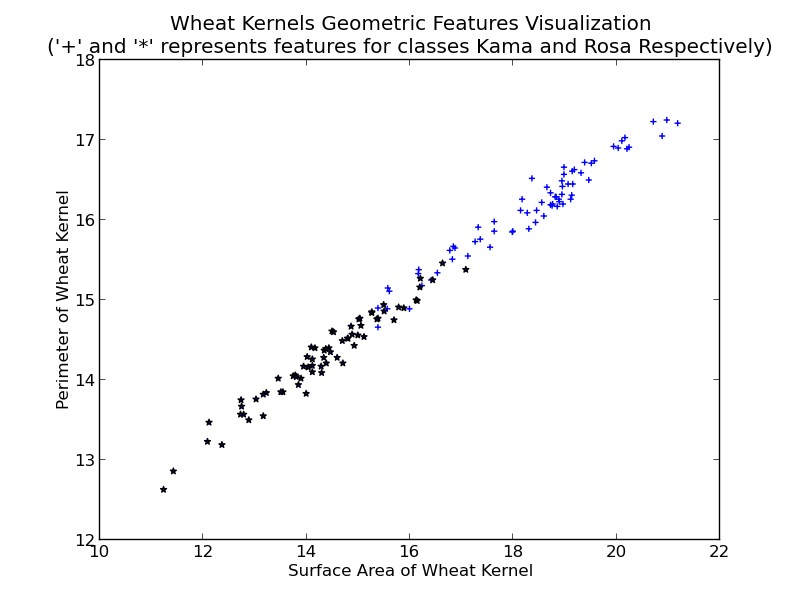
\includegraphics[width=0.6\textwidth]{pics/FeaturesVisualization.png} 
    \caption{Dataset Features Visualization}
    \label{fig:seeds}
\end{figure}

\section{Parametric Values for the Datasets}
\subsection{Mammographic dataset}
Mean For 2 classes :49.71317829, 62.25909091. \\
Standard deviation:185.59215191, 152.4828719. \\
The graph is same as the graph for Feature 2 in Figure \ref{fig:mam}.
\subsection{Wine dataset}
Mean:1115.71186441, 519.50704225. \\
Standard deviation: 48239.7305372, 24367.26403491.
The graph is same as the one in Figure \ref{fig:wine}.
\section{Computing best dichotomy parameters}
I used a modified binary search to find the right value for dichotomy, the code for which is present at: $\texttt{parametric\_est.py}$. Values for the 2 datasets is as shown below:
\subsection{Mammographic dataset}
Best feature Dichotomy value: 58.25.\\
\subsection{Wine dataset}
Best feature Dichotomy value: 980.37109375.\\
\section{Classification Accuracy}
The accuracy for different values of n for n-fold validation on different datasets is shown below:
\subsection{Wine dataset}
The results for different values of n are as shown in Table \ref{tab:wine}
\begin{table}
\centering
\begin{tabular}{ | c | c |}
    \hline
    {\bf N} & {\bf Mean Accuracy} \\ 
    \hline
    3 & 0.923\\
	\hline
	4 & 0.931\\
	\hline
	5 & 0.923\\
	\hline
	6 & 0.922\\
	\hline
	7 & 0.923\\
	\hline
	8 & 0.923\\
	\hline
	9 & 0.923\\
	\hline
	10 & 0.923\\
	\hline
	\end{tabular}
	\caption{Cross Validation Results for Wine}
    \label{tab:wine}
\end{table}
\subsection{Mammographic dataset}
The results for different values of n are as shown in Table \ref{tab:man}
\begin{table}
\centering
\begin{tabular}{ | c | c |}
    \hline
    {\bf N} & {\bf Mean Accuracy} \\ 
    \hline
    3 & 0.672\\
	\hline
	4 & 0.678\\
	\hline
	5 & 0.671\\
	\hline
	6 & 0.678\\
	\hline
	7 & 0.677\\
	\hline
	8 & 0.678\\
	\hline
	9 & 0.676\\
	\hline
	10 & 0.676\\
	\hline
	\end{tabular}
	\caption{Cross Validation Results for Mammographic}
    \label{tab:man}
\end{table}
\end{document}